% Task 1.3 -- Đặc tả use-case "Đặt và thanh toán đơn hàng"
% File chỉ chứa nội dung theo quy ước; trang bìa, header/footer nằm ở report.tex (ngoài repo).

\subsection{Task 1.3 -- Đặc tả use-case Đặt và thanh toán đơn hàng}

Mục này đặc tả chi tiết use-case quan trọng nhất của BrewLite: khách hàng đặt đơn từ giỏ hàng và thanh toán không dùng tiền mặt.
Use-case này gộp các use-case UC-03 đến UC-06, UC-09 đến UC-11 trong sơ đồ tổng quát (Task~1.2) thành một luồng đi từ lúc bấm \emph{Đặt hàng} đến khi khách nhìn thấy màn hình xác nhận đơn.
Đặc tả bám đúng hành vi của hệ thống đã cài đặt ở Assignment~1 và máy trạng thái đơn hàng (đề A1, mục 9.1).

Hệ thống không kết nối cổng thanh toán thật.
Vai trò ``cổng thanh toán giả lập'' do \textbf{Ngân hàng giả lập} đảm nhận: khách quét mã QR, bấm \emph{Chuyển tiền}, tiền được ghi vào sao kê của quán.
Theo yêu cầu của giảng viên, hệ thống \textbf{không tự đánh dấu đơn đã thanh toán}: chỉ nhân viên (\texttt{ADMIN}) sau khi đối chiếu sao kê mới chuyển đơn sang \texttt{PAID}.
Vì vậy hệ thống không có bước ``callback từ cổng thanh toán''; quyền xác nhận thanh toán được bảo vệ bằng phân quyền \texttt{ADMIN} thay cho chữ ký callback.

% -------------------------------------------------------------------------
\subsubsection{Sơ đồ use-case}

\begin{figure}[htbp]
  \centering
  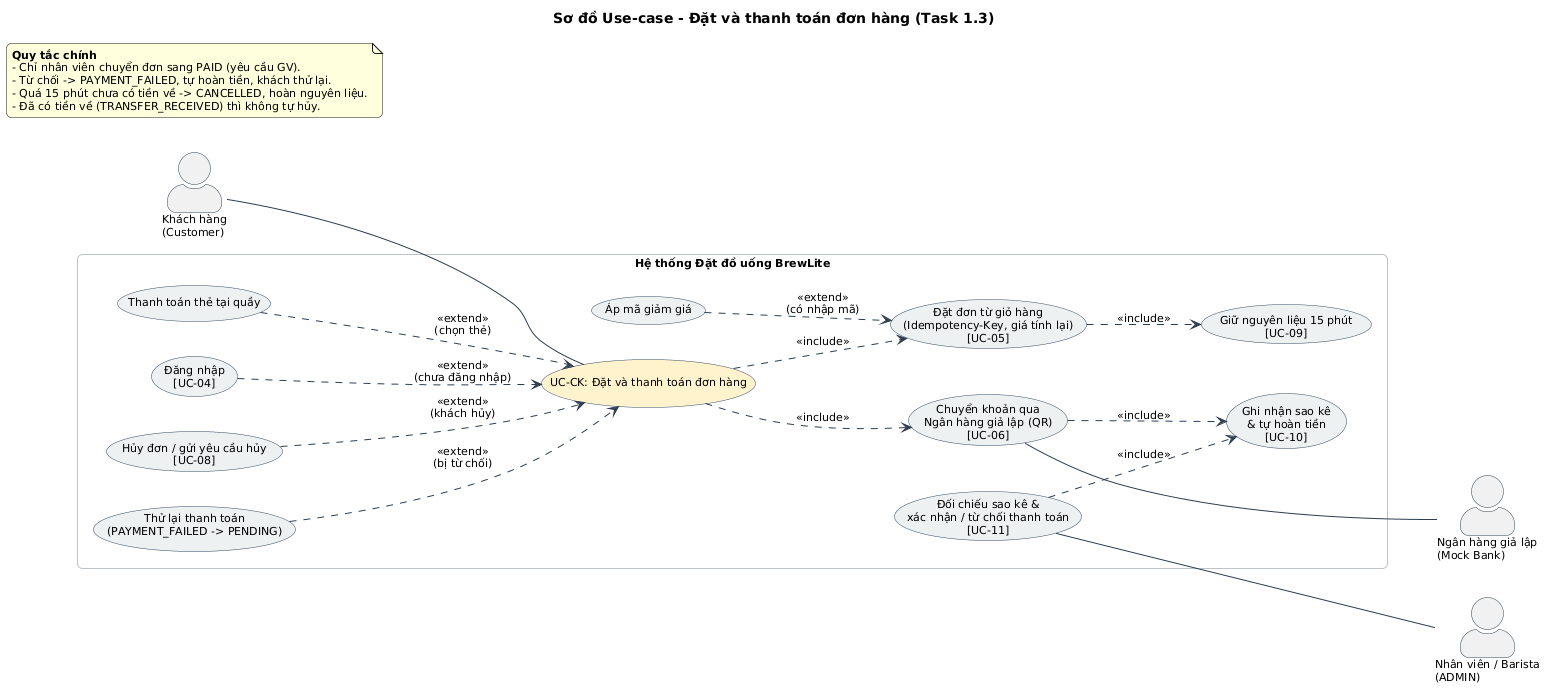
\includegraphics[width=0.95\textwidth]{docs/diagrams/usecase-checkout.png}
  \caption{Sơ đồ use-case ``Đặt và thanh toán đơn hàng''}
  \label{fig:usecase-checkout}
\end{figure}

Hình~\ref{fig:usecase-checkout} cho thấy use-case chính \textbf{UC-CK: Đặt và thanh toán đơn hàng} luôn bao gồm (\texttt{<<include>>}) việc tạo đơn, giữ nguyên liệu, chuyển khoản qua ngân hàng giả lập và ghi nhận sao kê.
Các tình huống chỉ xảy ra trong một số trường hợp (đăng nhập, áp mã giảm giá, quẹt thẻ tại quầy, thử lại thanh toán, hủy đơn) được vẽ là \texttt{<<extend>>}.
Nhân viên tham gia qua use-case \emph{Đối chiếu sao kê \& xác nhận thanh toán}.

% -------------------------------------------------------------------------
\subsubsection{Thông tin chung}

\begin{longtable}{@{}p{3.6cm}p{12.4cm}@{}}
\toprule
\textbf{Mục} & \textbf{Nội dung} \\
\midrule
\endhead
Mã use-case & UC-CK \\
Tên & Đặt và thanh toán đơn hàng \\
Actor chính & Khách hàng (tài khoản \texttt{CUSTOMER}) \\
Actor phụ &
  \begin{itemize}[leftmargin=*]
    \item \textbf{Ngân hàng giả lập}: đóng vai cổng thanh toán giả lập, nhận lệnh chuyển tiền và ghi vào sao kê của quán.
    \item \textbf{Nhân viên / Barista} (tài khoản \texttt{ADMIN}): đối chiếu sao kê, xác nhận hoặc từ chối thanh toán.
  \end{itemize} \\
Trigger & Khách bấm nút \emph{Đặt hàng} trên trang giỏ hàng (\texttt{/cart}). \\
Tiền điều kiện &
  \begin{itemize}[leftmargin=*]
    \item Giỏ hàng có ít nhất một món; mỗi món đã chọn size và topping hợp lệ.
    \item Món và topping đã có công thức nguyên liệu trong cơ sở dữ liệu.
    \item Hệ thống (frontend, backend, PostgreSQL) đang hoạt động.
    \item Khách chưa cần đăng nhập trước: nếu chưa đăng nhập, luồng thay thế A1 xử lý.
  \end{itemize} \\
Hậu điều kiện (thành công) &
  \begin{itemize}[leftmargin=*]
    \item Đơn ở trạng thái \texttt{PAID}; phiên thanh toán ở trạng thái \texttt{SUCCESS}.
    \item Sao kê của quán có đúng một giao dịch tiền vào (\texttt{IN}) bằng tổng tiền đơn.
    \item Nguyên liệu đã giữ khi tạo đơn được trừ hẳn khỏi kho; không trừ thêm khi thanh toán.
    \item Lượt dùng mã giảm giá (nếu có) được chốt; khách được cộng điểm thưởng.
    \item Giỏ hàng được xóa; khách thấy màn hình xác nhận đơn; đơn xuất hiện trên bảng pha chế.
  \end{itemize} \\
Hậu điều kiện (thất bại) &
  \begin{itemize}[leftmargin=*]
    \item Không có đơn nào được tạo (lỗi khi đặt đơn), hoặc đơn ở \texttt{PAYMENT\_FAILED} (chờ khách thử lại) hay \texttt{CANCELLED}.
    \item Đơn \texttt{CANCELLED}: nguyên liệu được hoàn về kho đúng một lần, lượt mã giảm giá được trả lại.
    \item Mọi khoản tiền đã nhận của đơn bị từ chối hoặc bị hủy đều được tự động hoàn trên sao kê.
    \item Giỏ hàng được giữ nguyên để khách đặt lại.
  \end{itemize} \\
Yêu cầu liên quan & FR-03, FR-04, FR-05, FR-06, FR-07, FR-08, FR-09, FR-10, FR-13; NFR-01, NFR-02, NFR-03 (theo SRS Task~1.2) \\
\bottomrule
\end{longtable}

% -------------------------------------------------------------------------
\subsubsection{Luồng chính}

Luồng chính mô tả trường hợp khách đã đăng nhập, đủ nguyên liệu, thanh toán bằng chuyển khoản qua ngân hàng giả lập và được nhân viên xác nhận.

\begin{longtable}{@{}p{0.8cm}p{5.4cm}p{9.8cm}@{}}
\toprule
\textbf{Bước} & \textbf{Actor} & \textbf{Hệ thống} \\
\midrule
\endhead
1 & Khách hàng bấm \emph{Đặt hàng} trên trang giỏ hàng (có thể nhập mã giảm giá).
  & Giao diện kiểm tra đã đăng nhập, gửi \texttt{POST /orders} kèm JWT, header \texttt{Idempotency-Key} và danh sách món (sản phẩm, size, topping, số lượng). \\
2 & ---
  & Backend kiểm tra JWT và dữ liệu gửi lên. Trong \textbf{một transaction}: lưu \texttt{Idempotency-Key}; tính lại đơn giá từ cơ sở dữ liệu (size M +5.000đ, size L +10.000đ, mỗi topping +5.000đ), không tin giá từ client; áp mã giảm giá và giữ lượt dùng; giữ nguyên liệu theo công thức (size M $\times 1{,}25$, size L $\times 1{,}5$, topping trừ riêng) bằng \emph{optimistic locking}; tạo đơn \texttt{PENDING} với hạn thanh toán 15 phút. Trả về HTTP 201 gồm mã đơn, tổng tiền, trạng thái và hạn thanh toán. Giỏ hàng vẫn được giữ. \\
3 & Khách hàng chọn phương thức thanh toán \emph{Chuyển khoản / Ví} trên trang \texttt{/checkout/:orderId}.
  & Giao diện hiển thị tổng tiền và đồng hồ đếm ngược hạn thanh toán. \\
4 & ---
  & Giao diện gửi \texttt{POST /payments} (mã đơn, phương thức \texttt{WALLET}) kèm \texttt{Idempotency-Key}. Backend kiểm tra đơn thuộc về khách, đơn đang \texttt{PENDING} và còn hạn; tạo phiên thanh toán \texttt{PENDING} với số tiền lấy từ đơn. Giao diện chuyển sang trang \texttt{/pay/:paymentId} và hiển thị mã QR. \\
5 & Khách hàng dùng điện thoại quét mã QR.
  & Trang Ngân hàng giả lập (\texttt{/mock-bank/:paymentId}) hiển thị số tiền cố định và nội dung chuyển khoản là mã đơn; trang này không cần đăng nhập. \\
6 & Khách hàng bấm \emph{Chuyển tiền}.
  & Ngân hàng giả lập ghi một giao dịch tiền vào (\texttt{IN}) trên sao kê của quán và chuyển phiên sang \texttt{TRANSFER\_RECEIVED}. Đơn \textbf{vẫn ở} \texttt{PENDING}; từ lúc này đơn không bị tự hủy khi quá hạn vì khách đã trả tiền đúng hạn. \\
7 & Nhân viên mở tab \emph{Thanh toán} trên trang quản trị.
  & Trang quản trị tự làm mới mỗi 4 giây, phát thông báo và âm báo khi có tiền về, đưa phiên có tiền về lên đầu danh sách. \\
8 & Nhân viên đối chiếu sao kê (số tiền, nội dung là mã đơn) và bấm \emph{Xác nhận}.
  & Backend khóa dòng phiên và đơn (\emph{pessimistic locking}), chuyển phiên sang \texttt{SUCCESS} và đơn \texttt{PENDING} $\rightarrow$ \texttt{PAID} qua \texttt{assertTransition}; chốt lượt mã giảm giá; cộng điểm thưởng (mỗi 10.000đ thực trả $= 1$ điểm, làm tròn xuống). \\
9 & ---
  & Giao diện của khách hỏi lại trạng thái phiên định kỳ (\texttt{GET /payments/:id}); khi thấy đơn \texttt{PAID} thì xóa giỏ hàng và chuyển sang \texttt{/orders/:id/confirmation}. \\
10 & Khách hàng xem màn hình xác nhận.
  & Hiển thị mã đơn, trạng thái \texttt{PAID}, danh sách món, giảm giá và tổng tiền. Use-case kết thúc; đơn chuyển sang bảng pha chế (UC-13, ngoài phạm vi use-case này). \\
\bottomrule
\end{longtable}

% -------------------------------------------------------------------------
\subsubsection{Luồng thay thế}

\begin{longtable}{@{}p{0.8cm}p{3.6cm}p{11.6cm}@{}}
\toprule
\textbf{Mã} & \textbf{Điều kiện} & \textbf{Mô tả} \\
\midrule
\endhead
A1 & Chưa đăng nhập (bước 1)
  & Giao diện chuyển sang \texttt{/login?redirect=/cart}. Khách đăng nhập (hoặc đăng ký rồi đăng nhập); hệ thống quay lại giỏ hàng, giỏ còn nguyên nhờ lưu trong \texttt{localStorage}. Tiếp tục từ bước 1. Nếu gọi thẳng API không có JWT, backend trả HTTP 401. \\
A2 & Thanh toán bằng thẻ tại quầy (bước 3--8)
  & Khách chọn \emph{Thẻ tại quầy} (\texttt{CARD}); mã QR trên trang thanh toán là mã đơn để nhân viên tra cứu. Khách đưa thẻ cho nhân viên quẹt bên ngoài hệ thống. Nhân viên bấm \emph{Xác nhận}: hệ thống ghi giao dịch tiền vào ``Quẹt thẻ tại quầy'' trên sao kê rồi làm tiếp như bước 8. \\
A3 & Nhân viên từ chối thanh toán (bước 8)
  & Nhân viên bấm \emph{Từ chối} (ví dụ số tiền hoặc nội dung không khớp). Phiên chuyển \texttt{FAILED}, đơn \texttt{PENDING} $\rightarrow$ \texttt{PAYMENT\_FAILED}; hệ thống tự ghi giao dịch hoàn tiền (\texttt{REFUND}) đúng số đã nhận. Giỏ hàng giữ nguyên; giao diện báo thanh toán thất bại và cho chọn \emph{Thử lại} hoặc về giỏ hàng. Nguyên liệu vẫn được giữ cho đơn. \\
A4 & Khách thử lại sau khi bị từ chối
  & Giao diện gửi \texttt{POST /payments} với \texttt{Idempotency-Key} mới. Backend chuyển đơn \texttt{PAYMENT\_FAILED} $\rightarrow$ \texttt{PENDING} rồi tạo phiên thanh toán mới; tiếp tục từ bước 4. Hệ thống \textbf{không bao giờ} chuyển thẳng \texttt{PAYMENT\_FAILED} $\rightarrow$ \texttt{PAID}. Hạn thanh toán vẫn tính từ lúc tạo đơn, không được gia hạn. \\
A5 & Gửi lặp cùng \texttt{Idempotency-Key} (bước 1, bước 4)
  & Khách bấm nhiều lần, mạng chập chờn hoặc trình duyệt gửi lại. \texttt{POST /orders} cùng key và cùng giỏ hàng: trả về đúng đơn cũ, không tạo đơn mới, không giữ nguyên liệu lần hai. Cùng key nhưng giỏ hàng khác: HTTP 409. \texttt{POST /payments} cùng key: trả về đúng phiên cũ, không tạo phiên mới. Giao diện dùng lại key cũ cho tới khi đơn được tạo xong. \\
A6 & Khách đổi phương thức khi phiên còn \texttt{PENDING}
  & Hệ thống cập nhật phương thức trên phiên hiện có, không tạo phiên thứ hai cho cùng một đơn. \\
A7 & Khách hủy đơn trong lúc chờ thanh toán
  & Đơn chưa có tiền về: khách bấm \emph{Hủy đơn}, đơn chuyển \texttt{CANCELLED}, hoàn nguyên liệu và lượt mã giảm giá. Đơn đã có tiền về hoặc đã \texttt{PAID} (chưa pha chế): khách chỉ gửi được \emph{yêu cầu hủy}; nhân viên duyệt thì đơn chuyển \texttt{CANCELLED} và hệ thống tự hoàn đúng số tiền đã nhận (UC-08, UC-12). \\
\bottomrule
\end{longtable}

% -------------------------------------------------------------------------
\subsubsection{Luồng ngoại lệ}

\begin{longtable}{@{}p{0.8cm}p{3.6cm}p{11.6cm}@{}}
\toprule
\textbf{Mã} & \textbf{Điều kiện} & \textbf{Mô tả} \\
\midrule
\endhead
E1 & Không đủ nguyên liệu (bước 2)
  & Transaction bị hủy toàn bộ (rollback), backend trả HTTP 400 ``<tên nguyên liệu> không đủ nguyên liệu''. Không tạo đơn, không giữ nguyên liệu, không giữ lượt mã giảm giá; giỏ hàng giữ nguyên. Khi nhiều khách cùng đặt món chỉ còn đủ cho một ly, chỉ một đơn thành công (NFR-01). \\
E2 & Dữ liệu đặt đơn không hợp lệ (bước 1--2)
  & Giỏ hàng rỗng, size hoặc số lượng sai: HTTP 400. Sản phẩm không tồn tại: HTTP 400. Thiếu header \texttt{Idempotency-Key}: HTTP 400. Không tạo đơn. \\
E3 & Mã giảm giá không hợp lệ (bước 2)
  & Mã không tồn tại, hết hạn hoặc tài khoản đã dùng đủ 3 lần: backend báo lỗi và không tạo đơn; khách bỏ hoặc đổi mã rồi đặt lại. \\
E4 & Quá 15 phút chưa có tiền về
  & Tác vụ nền quét mỗi 5 giây chuyển đơn \texttt{PENDING} hoặc \texttt{PAYMENT\_FAILED} sang \texttt{CANCELLED} (lý do hết hạn thanh toán), hoàn nguyên liệu đúng một lần và trả lượt mã giảm giá. Thao tác thanh toán sau đó bị từ chối với thông báo ``Đơn đã hết hạn hoặc bị hủy''. Đơn đã có tiền về (\texttt{TRANSFER\_RECEIVED}) \textbf{không} bị tự hủy. \\
E5 & Yêu cầu xác nhận thanh toán không hợp lệ (bước 6, 8)
  & Thay cho kiểm tra chữ ký callback: tài khoản không phải \texttt{ADMIN} gọi API xác nhận/từ chối bị HTTP 403, nên khách không thể tự đánh dấu \texttt{PAID}. Chuyển tiền cho phiên đã xử lý hoặc đơn không còn \texttt{PENDING}: HTTP 400. Hai nhân viên cùng bấm hoặc bấm lặp: khóa dòng bảo đảm chỉ một lần được xử lý, tiền không bị ghi hay hoàn hai lần. Đơn đang chờ duyệt hủy: không xác nhận được thanh toán (HTTP 409). \\
E6 & Thanh toán đơn của người khác (bước 4)
  & Backend trả HTTP 403 và không tạo phiên. Xem chi tiết đơn của người khác trả HTTP 404 để không lộ sự tồn tại của đơn. \\
E7 & Lỗi kết nối hoặc lỗi máy chủ
  & Giao diện hiển thị thông báo lỗi kèm nút \emph{Thử lại}; giỏ hàng giữ nguyên. Lần thử lại dùng cùng \texttt{Idempotency-Key} nên nếu yêu cầu trước đã thành công thì không phát sinh đơn hay phiên trùng. \\
\bottomrule
\end{longtable}

% -------------------------------------------------------------------------
\subsubsection{Trạng thái đơn trong use-case}

Mọi thay đổi trạng thái đều đi qua \texttt{assertTransition}, khớp sơ đồ máy trạng thái của đề A1 (mục 9.1).
Chuyển trạng thái không có trong bảng dưới bị từ chối với HTTP 400.

\begin{longtable}{@{}p{5.2cm}p{4.6cm}p{6.2cm}@{}}
\toprule
\textbf{Chuyển trạng thái} & \textbf{Xảy ra ở} & \textbf{Ai / khi nào} \\
\midrule
\endhead
(tạo mới) $\rightarrow$ \texttt{PENDING} & Bước 2 & Khách đặt đơn thành công \\
\texttt{PENDING} $\rightarrow$ \texttt{PAID} & Bước 8, A2 & Nhân viên xác nhận thanh toán \\
\texttt{PENDING} $\rightarrow$ \texttt{PAYMENT\_FAILED} & A3 & Nhân viên từ chối thanh toán \\
\texttt{PAYMENT\_FAILED} $\rightarrow$ \texttt{PENDING} & A4 & Khách thử lại thanh toán \\
\texttt{PENDING} / \texttt{PAYMENT\_FAILED} $\rightarrow$ \texttt{CANCELLED} & A7, E4 & Khách hủy (chưa có tiền về) hoặc hết hạn 15 phút \\
\texttt{PAID} $\rightarrow$ \texttt{CANCELLED} & A7 & Nhân viên duyệt yêu cầu hủy, hệ thống hoàn tiền \\
\bottomrule
\end{longtable}

Phiên thanh toán có trạng thái riêng: \texttt{PENDING} (chờ tiền) $\rightarrow$ \texttt{TRANSFER\_RECEIVED} (tiền đã về, chờ nhân viên) $\rightarrow$ \texttt{SUCCESS} (đã xác nhận) hoặc \texttt{FAILED} (bị từ chối hoặc đơn bị hủy).
Trạng thái \texttt{TRANSFER\_RECEIVED} chỉ thuộc về phiên thanh toán, không phải trạng thái đơn, nên không làm thay đổi máy trạng thái của đề.

% -------------------------------------------------------------------------
\subsubsection{Hệ thống làm và không làm}

\paragraph{Hệ thống làm}
\begin{itemize}
  \item Tính lại giá, giữ nguyên liệu và tạo đơn trong một transaction; không bán vượt nguyên liệu.
  \item Giữ đơn chờ thanh toán tối đa 15 phút, quá hạn thì tự hủy và hoàn nguyên liệu.
  \item Ghi mọi khoản tiền vào và hoàn tiền trên sao kê của quán; tự hoàn tiền khi từ chối hoặc hủy đơn đã có tiền.
  \item Chống tạo trùng đơn và trùng phiên thanh toán bằng \texttt{Idempotency-Key}.
  \item Chỉ xóa giỏ hàng khi đơn đã \texttt{PAID}.
\end{itemize}

\paragraph{Hệ thống không làm}
\begin{itemize}
  \item Không kết nối ngân hàng, VNPay, MoMo hay cổng thanh toán thật; không nhận tiền mặt.
  \item Không tự đánh dấu \texttt{PAID} khi có tiền về; không có callback tự động từ cổng thanh toán.
  \item Không cho đặt đơn khi chưa đăng nhập; không tin giá do client gửi lên.
  \item Không gia hạn thời gian giữ nguyên liệu; không cho hủy đơn từ \texttt{PREPARING} trở đi.
  \item Không đổi điểm thưởng lấy đồ uống hay voucher (FR-15, ngoài phạm vi MVP).
\end{itemize}

% -------------------------------------------------------------------------
\subsubsection{Liên kết với yêu cầu}

\begin{longtable}{@{}p{2.2cm}p{5.0cm}p{8.8cm}@{}}
\toprule
\textbf{Mã} & \textbf{Yêu cầu} & \textbf{Bước / luồng trong UC-CK} \\
\midrule
\endhead
FR-03 & Quản lý giỏ hàng & Bước 1, 9; A1, A3 (giỏ giữ nguyên tới khi \texttt{PAID}) \\
FR-04 & Đăng ký \& đăng nhập & A1; E5 (phân quyền \texttt{ADMIN}) \\
FR-05 & Đặt đơn hàng & Bước 1--2; A5; E2 \\
FR-06 & Tồn kho theo nguyên liệu & Bước 2; A7, E1, E4 \\
FR-07 & Thanh toán qua ngân hàng giả lập \& thẻ & Bước 3--6; A2, A5, A6; E6 \\
FR-08 & Đối chiếu sao kê \& xác nhận thanh toán & Bước 7--8; A3; E5 \\
FR-09 & Hủy đơn \& hoàn tiền & A7 \\
FR-10 & Máy trạng thái \& tự hủy quá hạn & Bước 2, 8; A3, A4; E4 \\
FR-13 & Khuyến mãi \& điểm thưởng & Bước 1, 2, 8; E3 \\
NFR-01 & Hiệu năng \& xử lý đồng thời & Bước 2; A5; E1 \\
NFR-02 & Bảo mật & Bước 2, 8; E5, E6 \\
NFR-03 & Tính khả dụng & Bước 3, 9--10; E7 \\
\bottomrule
\end{longtable}
